\chapter{大きさについて (On Magnitude)}

\section{大きさの幾何学と物理的次元}

自然の探求において、われわれはあらゆる知覚と観察を「大きさ（Magnitude）」と「方向（Direction）」という概念に還元しなければならない。物理学におけるすべての物理量は、長さ $[L]$、質量 $[M]$、時間 $[T]$ という基本次元によって構成される。

幾何学の世界において、ユークリッド空間の相似な図形は、その絶対的な大きさとは無関係に同一の比率と角度を保つ。相似三角形の角度は、その辺が1ミリメートルであろうと1光年であろうと完全に等しい。しかし、物理的・物質的な世界においては、**「絶対的な大きさ（Absolute Magnitude）」**が決定的な意味を持つ。なぜなら、物質には質量があり、重力、弾性、粘性、表面張力といった物理的な力が、長さの異なる次元（累乗）に比例して作用するからである。

\section{2乗3乗則の力学的帰結}

長さを $L$ とする相似な立体において、表面積 $S$ は $L^2$ に比例し、体積 $V$ は $L^3$ に比例する：
\begin{align}
    S &\propto L^2 \\
    V &\propto L^3
\end{align}
密度が一様であるならば、質量および重量 $W$ もまた体積に比例して $W \propto L^3$ となる。

この**「2乗3乗則（Square-Cube Law）」**は、ガリレオ・ガリレイが1638年の『新科学対話』において初めて明確に指摘した自然界の鉄則である。この幾何学的原理から、直ちに以下の力学的制約が導かれる：

\subsection{1. 骨格の支持力と断面積}
動物の体重を支える骨の強度（耐荷重能）は、骨の体積ではなく、その**横断面積（$A \propto L^2$）**に比例する。
もしある動物の身体の長さのすべての寸法を一様に $k$ 倍（例えば $k=10$ 倍）にしたと仮定しよう。
\begin{itemize}
    \item 骨の断面積は $k^2 = 100$ 倍になる。
    \item 身体の体重は $k^3 = 1000$ 倍になる。
\end{itemize}
したがって、骨の単位断面積あたりにかかる圧縮応力 $\sigma$ は、
\begin{equation}
    \sigma = \frac{W}{A} \propto \frac{L^3}{L^2} = L
\end{equation}
となり、長さ $L$ に正比例して増大する。相似な形のまま10倍に巨大化すれば、骨は10倍もの激しい荷重を受け、自重に耐えかねて骨折してしまう。

これが、**「相似な形のままでの巨大生物の生存不可能性」**の数学的証明である。ガリレオが喝破したように、巨大な動物は小さな動物の相似拡大ではあり得ない。体重の増大を支えるためには、骨格は不釣り合いなほど太く重厚にならなければならず、ガゼルやシカの優美な脚は、ゾウやサイにおいては太い円柱状の柱へと変貌せざるを得ない。

\subsection{2. 熱放散と呼吸の表面積比}
動物の代謝活動によって産生される熱量は、体積（$L^3$）に比例する。一方、外界への熱放散は、体表面積（$L^2$）を通して行われる。
単位体重あたりの放熱面積は、
\begin{equation}
    \frac{S}{V} \propto \frac{L^2}{L^3} = \frac{1}{L}
\end{equation}
となり、体の大きさに反比例する。
ハツカネズミやハチドリのような微小な恒温動物は、体重に比して莫大な表面積を持つため、常に急速な熱損失に晒されている。彼らが体温を維持するためには、昼夜を問わず自身の体重に匹敵する食料を摂取し、極めて高い代謝率で熱を産生し続けなければならない。逆に、ゾウやクジラのような巨大動物は熱が逃げにくく、過熱（熱鬱滞）の危機に直面するため、巨大な耳（ゾウの放熱板）や特殊な血管網を発達させる必要がある。

\section{微小生物と表面張力の帝国}

生物の寸法が小さくなるにつれて、力学的支配権の劇的な交代が起こる。
体積に比例する重力（$W \propto L^3$）は急速に減衰し、表面積や長さに比例する力、とりわけ**表面張力（Surface Tension, $F_T \propto L$）**や流体の粘性抵抗が全能の支配者となる。

\begin{figure}[htbp]
    \centering
    \ifdefined\figplaceholder
    \else
    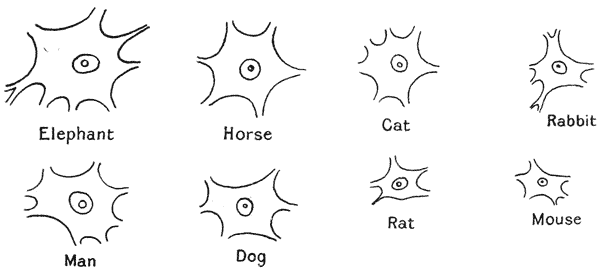
\includegraphics[width=0.45\textwidth]{images/i037.png}
    \fi
    \caption{微小液滴および表面張力による力学的平衡}
    \label{fig:surface_tension}
\end{figure}

人間が水に入るとき、表面張力は体感できないほど微小な力である。しかし、体長数ミリメートルのアリや昆虫にとって、水滴の表面張力は自重の数百倍から数千倍に達する恐るべき力である。水滴に触れた昆虫は、強力な粘着トラップに捕らえられたかのように身動きが取れなくなる。逆に、アメンボはこの表面張力を利用して水面上を沈むことなく疾走する。

\begin{figure}[htbp]
    \centering
    \ifdefined\figplaceholder
    \else
    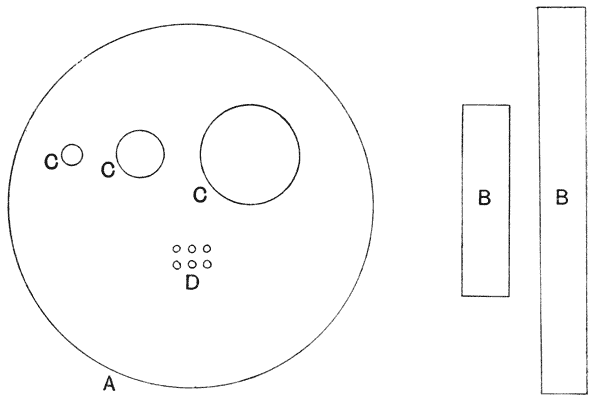
\includegraphics[width=0.45\textwidth]{images/i039.png}
    \fi
    \caption{重力と毛細管張力の釣り合い}
    \label{fig:capillary}
\end{figure}

さらに小さな単細胞生物（繊毛虫や細菌）の世界では、慣性力（$m a \propto L^4$）はほぼ完全に消失し、低レイノルズ数の粘性流動環境（ストークス流れの世界）となる。彼らにとって水はさらさらした液体ではなく、人間にとっての濃厚な水飴や蜂蜜のように粘り気のある媒体である。そこでは運動を止めた瞬間に慣性による滑空は一切なく、ただちに静止する。

\section{落下の物理学 --- ジョナサン・スウィフトの巨人国と自然の摂理}

『ガリヴァー旅行記』のブロブディンナグ（巨人国）に登場する60フィート（通常の10倍）の巨人は、物理学的に存在し得ない。彼らが転倒したとき、頭部が地面に衝突する衝撃エネルギーは自重と落差の積（$W \times h \propto L^3 \times L = L^4$）に比例し、通常の人間（$L=1$）の実に1万倍に達するからである。

J. B. S. ホールデンの有名なエッセイ『適切な大きさについて』にも先立つトムソンの議論は明快である：
\begin{quote}
「ハツカネズミは千ヤードの鉱山の坑道へ投げ込まれても、底に軟らかい地面があれば、埃を払って無傷で走り去る。ネズミは死に、人間は骨折して砕け、馬は飛び散る。」
\end{quote}
空気抵抗（終末速度 $v_t \propto \sqrt{L}$）と衝突時の運動エネルギー（$E \propto L^4$）の二重のスケーリングが、生物の生存と行動様式をその絶対的サイズごとに厳密に決定しているのである。
